\section{Estructuras utilizadas en los archivos}

Como mencionamos en la Sección \ref{sec:indice2}, para guardar toda la información referente a la colección de documentos, utilizaremos 4 archivos.

Combinando los enfoques de \citet{Zhang:2008}, (\citeyear{Zhang:2008}) y de \citet[p.~107]{Buettcher2010}, (\citeyear{Buettcher2010}), llegamos a las estructuras de archivos que describiremos.


\subsection{Los archivos flacos}

Estos archivos solamente almacenan un tipo de dato muy específico:

\begin{itemize}

\item \textbf{*.dic}: aquí se guardan todas los términos que se encontraron en la colección, una larga cadena con los mismos, separados con barra <</>> o espacio. Se los comprime con LZW, en bloques o bien se testeará con todo el archivo. 

\item \textbf{*.frq}: correspondientemente a cada término existe una frecuencia absoluta asociada, que se guarda en este archivo. Lógicamente son enteros sin orden distribuidos aleatoriamente. Se utilizará Rice coding, que es que mejor comprime, para conjuntos de frecuencias. Este archivo tiene la finalidad de ayudar a hacer las búsquedas más rápidas, ya que se irá filtrando por la palabra menos frecuente.

\item \textbf{*.ofs}: además se necesita guardar el offset (distancia) que existe para cierto término en el índice invertido. Como son enteros crecientes que se van a cargar en memoria principal, se utilizan deltas. Hay 2 opciones, o se comprime aplicando Rice coding o PFOR-Delta, separando en conjuntos de offsets, o se deja sin comprimir. Analizaremos si vale la pena el espacio se pierde con la última opción.


\begin{figure}[!h]
\centering
    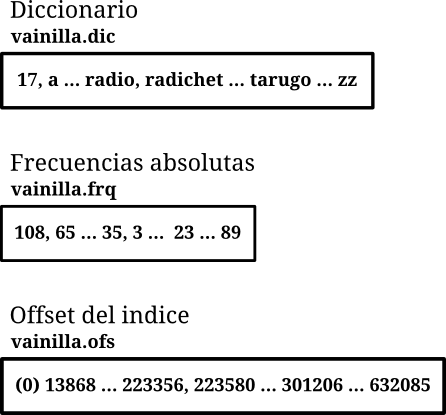
\includegraphics[scale=0.9]{./Images/estructura_2.png}
\caption{Los archivos flacos}
\label{fig:flacos}
\end{figure}



\end{itemize}

\subsection{El índice invertido}

El llamado índice invertido de posiciones sigue con total naturalidad lo propuesto por \cite{Zhang:2008}, pero sin bloques de tamaño de fijo, si no variables (en la frontera de los bytes).

La estructura general de nuestro índice invertido se muestra en la Figura \ref{fig:indice}. Se crean particiones en el archivo llamadas \textit{bloques}, de tamaño variable. 

\begin{figure}[h]
\centering
    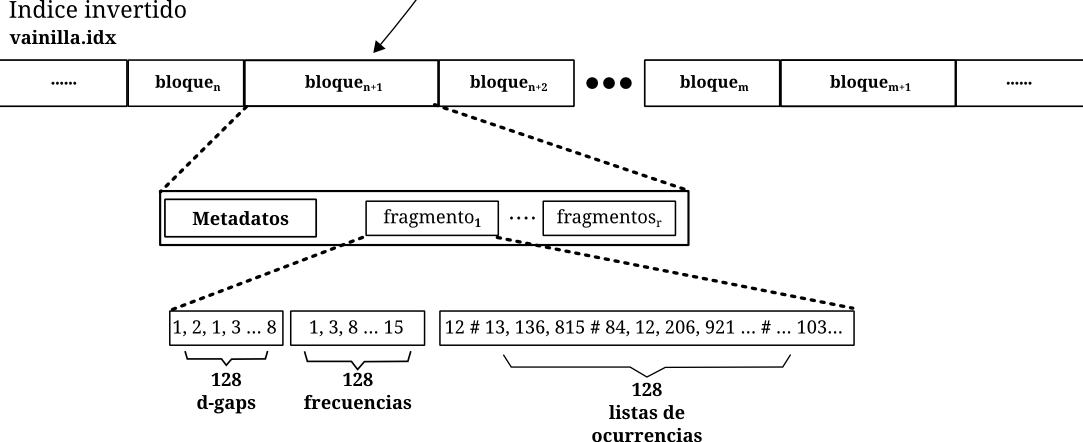
\includegraphics[scale=0.9]{./Images/estructura_1.png}
\caption{Estructura del índice invertido}
\label{fig:indice}
\end{figure}


Definimos un <<posteo>> como el conjunto de un docID, frecuencia relativa y lista de posiciones para un término (lógicamente, en un documento).

\paragraph{Un bloque}

\begin{itemize}

\item Guarda información correspondiente a un término de la colección.

\item Posee un gran número de listas invertidas correspondientes a las posiciones del término en consideración. Siguiendo con la referencia, dividimos estas listas en fragmentos con 128 posteos cada una. Este número podría cambiar para hacer más rápida la búsqueda en colecciones chicas o más grandes, pero siempre será múltiplo de 32.

\item Contiene metadatos (datos adicionales) con información de cuántos fragmentos posee y dónde comienzan (offset desde el primer fragmento), y a continuación los fragmentos. Esto se hace porque, como la estructura de datos permite decodificar los docIDs primero que lo demás, se quiere ser capaz de saltar al siguiente fragmento sin pasar por todos los datos comprimidos. No se decidió si comprimir los metadatos aún.

\end{itemize}

\paragraph{Un fragmento}

\begin{itemize}

\item Es una unidad básica para descomprimir datos en el índice invertido. Cada fragmento se puede descomprimir muy rápidamente.

\item Contiene 128 posteos almacenados como: 128 docIDs (almacenados como \textit{d-gaps}), luego 128 frecuencias relativas correspondientes y al final 128 listas de ocurrencias (guardadas como \textit{gaps} para cada docID). Los métodos de compresión serán, respectivamente, PFOR-Delta, Rice coding y PFOR-Delta nuevamente (a prueba, si no Rice coding).

\item Se lo puede <<saltar>> si el docID que buscamos no se encuentra, por ello este listado se comprime con PFOR-Delta (que guarda la el rango  máximo y el primer docID).

\end{itemize}
